%Version 2.1 April 2023 (Springer Nature template), filled for MapSORT
%
% Placeholders: \tbd marks a value still to be produced by a run; \figph marks a
% figure still to be made. Search for them before submission.

\documentclass[pdflatex,sn-basic]{sn-jnl}% author-year citations, as Precision Agriculture requires

\usepackage{graphicx}%
\usepackage{multirow}%
\usepackage{amsmath,amssymb,amsfonts}%
\usepackage{amsthm}%
\usepackage{mathrsfs}%
\usepackage[title]{appendix}%
\usepackage{xcolor}%
\usepackage{textcomp}%
\usepackage{manyfoot}%
\usepackage{booktabs}%
\usepackage{algorithm}%
\usepackage{algorithmicx}%
\usepackage{algpseudocode}%
\usepackage{geometry}%
\geometry{left=25mm,right=25mm,top=25mm,bottom=25mm,bindingoffset=0mm,headsep=5mm,footskip=10mm}
\usepackage{bm}%
\usepackage{tikz}%
\usetikzlibrary{arrows.meta,positioning,fit,backgrounds,calc,shapes.geometric}
\usepackage{pgfplots}%
\pgfplotsset{compat=1.18}

\theoremstyle{thmstyleone}%
\newtheorem{proposition}{Proposition}%

\raggedbottom

% ---- placeholders ----
\newcommand{\tbd}{{\color{gray}\scriptsize TBD}}
\newcommand{\figph}[3]{\fbox{\parbox[c][#2][c]{#1}{\centering\color{gray}\small #3}}}

% ---- notation ----
\newcommand{\bmu}{\bm{\mu}}
\newcommand{\bSig}{\bm{\Sigma}}
\newcommand{\bS}{\bm{S}}
\newcommand{\bX}{\bm{X}}
\newcommand{\bLam}{\bm{\Lambda}}
\newcommand{\bEta}{\bm{\eta}}
\newcommand{\hmu}{\hat{\bmu}}
\newcommand{\hSig}{\hat{\bSig}}
\newcommand{\RIP}{\mathrm{RIP}}

% ---- diagram colours ----
\definecolor{cmap}{RGB}{31,92,153}
\definecolor{capp}{RGB}{196,110,20}
\definecolor{clm}{RGB}{46,125,50}
\definecolor{ctrk}{RGB}{90,90,90}

\begin{document}

\title[MapSORT]{MapSORT: Landmark Association for Identity-Persistent Tracking of Stationary Crops and Fruit}

\author*[1]{\fnm{Srihari} \sur{Vemuru}}\email{vemshari27@gmail.com}

\affil*[1]{\orgdiv{\tbd}, \orgname{\tbd}, \orgaddress{\city{\tbd}, \country{\tbd}}}

\abstract{\textbf{Purpose:} Plant- and fruit-level records in precision agriculture, such as yield estimates, phenotyping logs and targeted spraying, require every plant or fruit to keep one identity across a video, including when the camera leaves and later returns to it. General-purpose multi-object trackers lose identity in exactly this situation, because crops look alike and an object out of view for more than a few frames is forgotten. This work turns the property that sets agricultural targets apart, that they do not move, into an association cue that keeps identities intact across occlusions and revisits.

\textbf{Methods:} MapSORT reconstructs the sequence with structure-from-motion and lifts every detection to a landmark observation: a Gaussian over the object's position in the scene map, with centre uncertainty kept separate from physical extent. Tracks fuse their observations in information form and are matched by a scale-invariant Mahalanobis gate inside a StrongSORT-style association cascade. Tracks that leave the view become dormant, not deleted, and are revived by their landmark. MapSORT is compared with BoT-SORT, SAM2MOT and StrongSORT on four public datasets (LettuceMOTS, MOrangeT, GrapeMOTS, AppleMOTS) and on per-tree yield counts in a mango orchard.

\textbf{Results:} MapSORT reaches \tbd{} HOTA and \tbd{} IDF1 on average, \tbd{} and \tbd{} points above the strongest baseline. It preserves identity in \tbd{}\% of revisit events, compared with \tbd{}\% for the best competitor. Per-tree mango counts are within \tbd{}\% of harvest counts. On a back-and-forth lettuce sequence MapSORT tracks all 37 plants with zero identity switches and an exact count.

\textbf{Conclusion:} A scene-map position is a persistent identity cue for stationary crops. Using it in association yields identity-consistent tracks and accurate counts across crops, platforms and viewing patterns.}

\keywords{Multi-object tracking, Structure-from-motion, Fruit counting, Plant re-identification, Agricultural robotics, Yield estimation}

\maketitle

%% =====================================================================
\section{Introduction}\label{sec:intro}

Many precision-agriculture tasks operate at the level of the individual plant or fruit. Yield estimation from video counts fruit by counting tracks \citep{stein2016mango,liu2019monocular,hani2020comparative,villacres2023apple}. Per-plant phenotyping attaches measurements from successive frames and passes to the same plant. Selective spraying and harvesting require an agricultural robot to know which plant it is looking at. All of these depend on multi-object tracking (MOT) that assigns each physical object one identity, and keeps it, for as long as the object is in the video.

Agricultural video makes this hard in a specific way. Plants in a row, oranges on a tree and grape bunches on a cane are visually near-identical, so appearance embeddings learned for pedestrians separate them poorly. Leaves, branches and neighbouring fruit occlude them. Most importantly, the camera routinely leaves an object and comes back to it: a ground robot drives a row and returns along it, a handheld camera sweeps the canopy more than once, a UAV inspects a vine from several perspectives. Tracking-by-detection methods \citep{bewley2016sort,wojke2017deepsort,zhang2022bytetrack,aharon2022botsort,du2023strongsort} predict object motion in the image plane and keep an unmatched track alive for a fixed number of frames. An object that is out of view for longer is deleted and receives a new identity when it reappears. Every such switch inflates the count and fragments the plant's record (Fig.~\ref{fig:teaser}).


The targets of agricultural tracking have a property that pedestrians and vehicles do not: they are stationary. A lettuce occupies the same place in the field on the outbound and return pass; an orange hangs at the same point of the canopy however often the camera sweeps past it. Its position in a three-dimensional map of the scene is therefore an identity cue that does not decay with time out of view, does not depend on appearance, and does not require the object's image-plane motion to be predictable. Structure-from-motion (SfM) recovers such a map, along with every camera pose, from the same monocular RGB video the tracker consumes \citep{schonberger2016colmap}.

\begin{figure}[b]
\centering
\figph{0.47\textwidth}{6.2cm}{\textbf{(a) BoT-SORT}\\[4pt]Return pass of LettuceMOTS 0011.\\Every returning plant carries a new identity;\\\tbd{} identities issued for 37 plants.}\hfill
\figph{0.47\textwidth}{6.2cm}{\textbf{(b) MapSORT}\\[4pt]Same frame.\\Every plant keeps the identity it received\\on the outbound pass; 37 identities issued.}
\caption{The same frame of a field robot's return pass along two lettuce rows, tracked by (a) BoT-SORT and (b) MapSORT. BoT-SORT has forgotten the plants it saw on the way out and counts each of them again. MapSORT recognises every plant from its position in the scene map and keeps one identity per plant.}
\label{fig:teaser}
\end{figure}

This paper presents MapSORT, a tracker that makes scene-map position a first-class association cue. MapSORT lifts each detection to a \emph{landmark observation}: a Gaussian over the object's centre in the map frame, with a covariance that expresses how well the centre is known and a separate extent that expresses how large the object is. Tracks accumulate their observations into a fused landmark whose uncertainty shrinks with every sighting. Association adds a landmark stage, gated by a Mahalanobis distance that is invariant to the arbitrary scale of a monocular reconstruction, to the appearance and motion stages of StrongSORT \citep{du2023strongsort}. A track that leaves the field of view is put to sleep rather than deleted, and is revived by its landmark when the camera returns, however long the absence.

The contributions of this work are:
\begin{enumerate}
\item A landmark observation model for detections of stationary objects, built from the SfM points the detection encloses, that separates centre uncertainty from object extent, fuses across observations in information form, and yields a gating distance invariant to reconstruction scale.
\item MapSORT, a tracking-by-detection method that inserts landmark association and landmark-based revival of dormant tracks into a StrongSORT association cascade, so that identity survives arbitrarily long absences.
\item A revisit-centred evaluation protocol: a revisit identity preservation rate that decomposes CLEAR identity switches by the absence that preceded them, together with count error, which is the quantity yield estimation consumes.
\item A benchmark against BoT-SORT, SAM2MOT and StrongSORT on four public agricultural datasets (LettuceMOTS, MOrangeT, GrapeMOTS and AppleMOTS), covering four crops, four platforms and three viewing patterns, and a yield-count evaluation in a mango orchard against harvested fruit counts per tree.
\end{enumerate}

%% =====================================================================
\section{Related work}\label{sec:related}

\subsection{Tracking-by-detection}

SORT \citep{bewley2016sort} established the tracking-by-detection template: a constant-velocity Kalman filter \citep{kalman1960} predicts each track's box, and Hungarian matching \citep{kuhn1955hungarian} on intersection-over-union (IoU) assigns detections to tracks. DeepSORT \citep{wojke2017deepsort} added an appearance embedding and a matching cascade that prioritises recently seen tracks. ByteTrack \citep{zhang2022bytetrack} recovers low-confidence detections in a second association round; OC-SORT \citep{cao2023ocsort} corrects Kalman drift during occlusion from observations; FairMOT \citep{zhang2021fairmot} learns detection and embedding jointly. BoT-SORT \citep{aharon2022botsort} combines camera-motion compensation, a refined Kalman state and fused IoU and appearance costs. StrongSORT \citep{du2023strongsort} modernises DeepSORT with a stronger re-identification backbone, exponential-moving-average feature updates, a noise-scaled Kalman filter and fused appearance and motion costs. SAM2MOT \citep{jiang2025sam2mot} departs from box association altogether: it uses the SAM~2 video segmentation model \citep{ravi2024sam2} to propagate object masks through time, so identity follows from segmentation rather than from matching.

All of these methods reason about identity in the image plane or in an appearance space. Neither is stable when the camera leaves an object and returns: image-plane motion over a long absence is not predictable, and appearance galleries are bounded in both size and age. MapSORT keeps the appearance and motion machinery of StrongSORT and adds a cue that remains valid over any absence.

\subsection{Tracking and counting in crops and orchards}

Video-based fruit counting tracks fruit to avoid counting it more than once. \citet{halstead2018fruit} tracked sweet pepper with IoU association on a robotic platform. \citet{hani2020comparative} compared detection and counting pipelines for apple yield mapping, and \citet{villacres2023apple} compared tracking-by-detection algorithms for apple production estimation. \citet{hu2022lettucemot} released LettuceMOT with back-and-forth and out-and-in robot trajectories and showed that re-occurring plants defeat standard trackers; the same group introduced LettuceMOTS with a shape-feature MOTS method for precision spraying \citep{hu2024lettucemots}. Datasets for homogeneous-object MOTS exist for apples \citep{dejong2022applemots} and grape bunches captured from multiple UAV perspectives \citep{arizasentis2024grapemots}, following the MOTS task definition of \citet{voigtlaender2019mots}.

\subsection{Three-dimensional localisation for fruit identity}

Several works use multi-view geometry to localise fruit. \citet{stein2016mango} triangulated mango detections from a GNSS/INS-referenced vehicle to count fruit per tree. \citet{liu2019monocular} combined monocular SfM with semantic data association to count and map fruit. \citet{genemola2020sfm} projected instance segmentations onto an SfM point cloud to locate apples in 3D. \citet{rapado2023tomato} tracked tomatoes in 3D from a robot arm with known camera poses. \citet{santos2024moranget} relocalised oranges in 3D to recover them after occlusion and showed that removing relocalisation more than halves HOTA on MOrangeT.

These approaches represent fruit position as a point and compare positions with a fixed, hand-tuned distance threshold. A point carries no notion of how well it is known, and a metric threshold is meaningless in a monocular reconstruction whose scale is arbitrary. MapSORT instead represents each observation as a Gaussian with an explicit covariance, fuses observations so that a track's position sharpens with every sighting, and gates association with a Mahalanobis distance that is independent of scale. It also integrates the landmark cue into a modern appearance-and-motion association cascade rather than replacing it, and uses it to revive tracks that a frame-to-frame tracker would have discarded.

%% =====================================================================
\section{Materials and methods}\label{sec:methods}

\subsection{Problem formulation}\label{sec:problem}

The input is a monocular RGB video $\{I_1,\dots,I_T\}$ captured by a moving camera, with no depth, odometry or positioning sensor, and at each frame $t$ a set of detections $D_t=\{d_t^1,\dots,d_t^{n_t}\}$, each an axis-aligned box $b_t^i$. The scene contains stationary objects. The task is to produce tracks $\mathcal{T}=\{\tau_1,\dots,\tau_K\}$, $\tau_k=\{(t,d_t^i)\}$, such that each track corresponds to exactly one physical object and each object to exactly one track: identity must be preserved through occlusion, visual ambiguity and camera motion, including when the camera returns to an object after it has been out of view.

\subsection{Overview}\label{sec:overview}

Fig.~\ref{fig:arch} shows the MapSORT pipeline. A scene map is reconstructed once per sequence by SfM (Sect.~\ref{sec:map}). At every frame, each detection receives an appearance embedding and a landmark observation read from the map (Sect.~\ref{sec:obs}). Tracks carry a Kalman state, an appearance gallery and a fused landmark (Sect.~\ref{sec:fusion}). A four-stage association cascade matches detections to active tracks by appearance and motion, by landmark, and by IoU, and finally to dormant tracks by landmark (Sect.~\ref{sec:assoc}). Tracks that leave the view are moved to a dormant pool instead of being deleted (Sect.~\ref{sec:dormant}). Algorithm~\ref{alg:mapsort} summarises one frame.

\begin{figure*}[t]
\centering
\resizebox{\textwidth}{!}{%
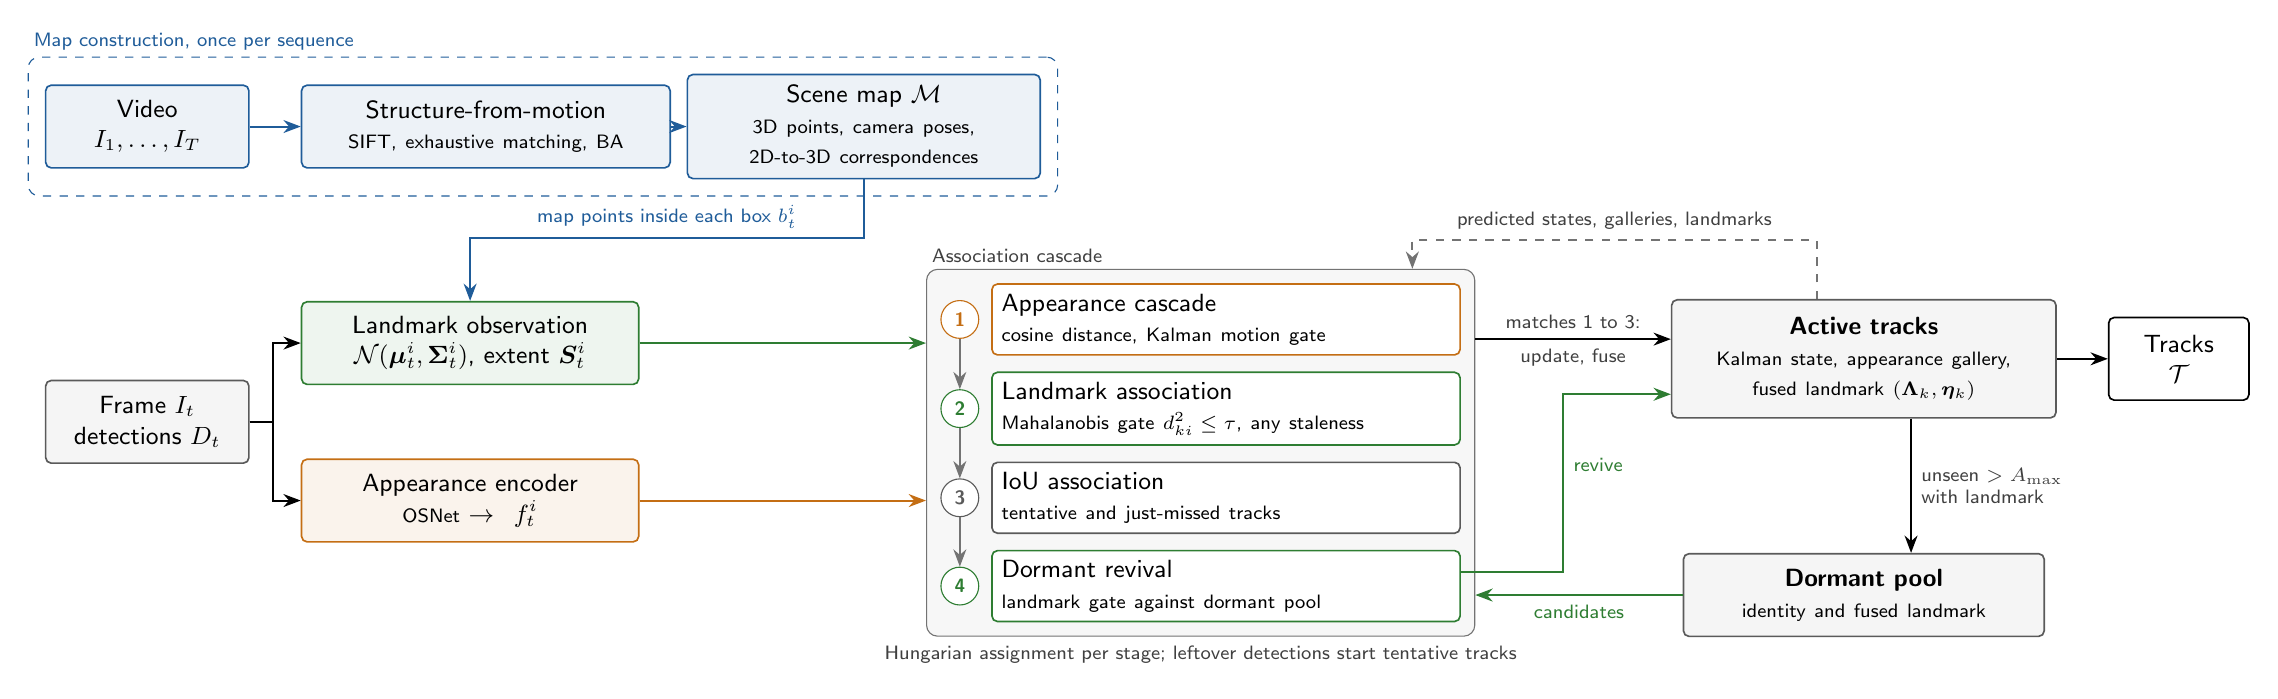
\begin{tikzpicture}[
  font=\sffamily\small,
  >={Stealth[length=2.2mm]},
  box/.style={draw, rounded corners=2pt, align=center, minimum height=1.05cm, inner sep=4pt, line width=0.6pt},
  mapbox/.style={box, draw=cmap, fill=cmap!8},
  appbox/.style={box, draw=capp, fill=capp!8},
  lmbox/.style={box, draw=clm, fill=clm!8},
  trkbox/.style={box, draw=ctrk, fill=ctrk!6},
  stage/.style={draw, rounded corners=2pt, align=left, text width=5.7cm, minimum height=0.85cm, inner sep=3.5pt, line width=0.6pt, fill=white},
  num/.style={circle, draw, fill=white, inner sep=0pt, minimum size=4.8mm, font=\sffamily\scriptsize\bfseries},
  lbl/.style={font=\sffamily\scriptsize, align=center, text=black!75},
  flow/.style={->, line width=0.7pt},
]
% ---------------- map construction ----------------
\node[mapbox, text width=2.3cm] (video) at (0,7.2) {Video\\$I_1,\dots,I_T$};
\node[mapbox, text width=4.4cm] (sfm) at (4.3,7.2) {Structure-from-motion\\{\scriptsize SIFT, exhaustive matching, BA}};
\node[mapbox, text width=4.2cm] (map) at (9.1,7.2) {Scene map $\mathcal{M}$\\{\scriptsize 3D points, camera poses, 2D-to-3D correspondences}};
\draw[flow, cmap] (video) -- (sfm);
\draw[flow, cmap] (sfm) -- (map);
\begin{scope}[on background layer]
\node[draw=cmap, dashed, rounded corners=4pt, fit=(video)(sfm)(map), inner sep=6pt, label={[lbl, text=cmap, anchor=south west, inner sep=2pt]north west:Map construction, once per sequence}] (mapgroup) {};
\end{scope}

% ---------------- per-frame inputs ----------------
\node[trkbox, text width=2.3cm] (frame) at (0,3.45) {Frame $I_t$\\detections $D_t$};
\node[lmbox, text width=4.0cm] (lm) at (4.1,4.45) {Landmark observation\\$\mathcal{N}(\bmu_t^i,\bSig_t^i)$, extent $\bS_t^i$};
\node[appbox, text width=4.0cm] (app) at (4.1,2.45) {Appearance encoder\\{\scriptsize OSNet} $\rightarrow f_t^i$};
\draw[flow] (frame.east) -- ++(0.3,0) |- (lm.west);
\draw[flow] (frame.east) -- ++(0.3,0) |- (app.west);
\draw[flow, cmap] (map.south) -- ++(0,-0.75) -| node[lbl, text=cmap, pos=0.25, above] {map points inside each box $b_t^i$} (lm.north);

% ---------------- association cascade ----------------
\node[stage, draw=capp] (s1) at (13.7,4.75) {Appearance cascade\\{\scriptsize cosine distance, Kalman motion gate}};
\node[stage, draw=clm, below=0.2cm of s1] (s2) {Landmark association\\{\scriptsize Mahalanobis gate $d^2_{ki}\le\tau$, any staleness}};
\node[stage, draw=ctrk, below=0.2cm of s2] (s3) {IoU association\\{\scriptsize tentative and just-missed tracks}};
\node[stage, draw=clm, below=0.2cm of s3] (s4) {Dormant revival\\{\scriptsize landmark gate against dormant pool}};
\foreach \s/\n/\c in {s1/1/capp, s2/2/clm, s3/3/ctrk, s4/4/clm}
  \node[num, draw=\c, text=\c, left=1.5mm of \s] (n\n) {\n};
\begin{scope}[on background layer]
\node[draw=black!55, rounded corners=4pt, fill=black!3, fit=(s1)(s4)(n1)(n4), inner sep=5pt, label={[lbl, anchor=north, inner sep=3pt]south:Hungarian assignment per stage; leftover detections start tentative tracks}] (casc) {};
\node[lbl, anchor=south west, inner sep=2pt] at (casc.north west) {Association cascade};
\end{scope}
\draw[flow, clm] (lm.east) -- (lm.east -| casc.west);
\draw[flow, capp] (app.east) -- (app.east -| casc.west);
\foreach \a/\b in {n1/n2, n2/n3, n3/n4}
  \draw[->, line width=0.5pt, black!55] (\a.south) -- (\b.north);

% ---------------- track store ----------------
\node[trkbox, text width=4.6cm, minimum height=1.5cm] (active) at (21.8,4.25) {\textbf{Active tracks}\\{\scriptsize Kalman state, appearance gallery, fused landmark $(\bLam_k,\bEta_k)$}};
\node[trkbox, text width=4.3cm] (dormant) at (21.8,1.25) {\textbf{Dormant pool}\\{\scriptsize identity and fused landmark}};
\node[box, draw=black, text width=1.5cm] (out) at (25.8,4.25) {Tracks\\$\mathcal{T}$};
\draw[flow] (active.east) -- (out.west);

\draw[flow] (s1.east |- active.west) ++(0,0.25) coordinate (m) (casc.east |- m) -- node[lbl, above] {matches 1 to 3:} node[lbl, below] {update, fuse} (active.west |- m);
\draw[flow, clm] ($(s4.east)+(0,0.18)$) -- ++(1.3,0) |- node[lbl, text=clm, pos=0.3, right] {revive} ($(active.west)+(0,-0.45)$);
\draw[flow, clm] (dormant.west) -- node[lbl, text=clm, below] {candidates} (dormant.west -| casc.east);
\draw[flow] ($(active.south)+(0.6,0)$) -- node[lbl, right, align=left] {unseen $>A_{\max}$\\with landmark} ($(dormant.north)+(0.6,0)$);
\draw[flow, dashed, black!55] ($(active.north)+(-0.6,0)$) |- ++(0,0.75) -| node[lbl, pos=0.25, above] {predicted states, galleries, landmarks} ($(casc.north east)+(-0.8,0)$);
\end{tikzpicture}}
\caption{MapSORT. A scene map is reconstructed once per sequence by structure-from-motion. At each frame, every detection gets an appearance embedding and a landmark observation: a Gaussian over its centre in the map frame, read from the map points it encloses. Detections are matched to active tracks by appearance and motion (1), by landmark (2) and by IoU (3), then to dormant tracks by landmark (4). Matched tracks fuse the new observation into their landmark. A confirmed track unseen for longer than $A_{\max}$ frames becomes dormant instead of being deleted, so a returning object reclaims its identity.}
\label{fig:arch}
\end{figure*}

\subsection{Scene map from structure-from-motion}\label{sec:map}

The scene map is a sparse SfM reconstruction of the sequence computed with COLMAP \citep{schonberger2016colmap}. SIFT features \citep{lowe2004sift} are extracted at full resolution, because the finest scale-space octaves carry the small objects, fruit and bunches, from which landmarks are read. All frames share one camera with a radial distortion model. Matching is exhaustive rather than sequential, so that frames from a revisit are matched directly to frames from the first pass and the two passes share 3D points; this is what places a returning object at the same map position. Incremental mapping with bundle adjustment then yields camera poses, a point cloud, and for every registered frame the 2D keypoints that observe each 3D point. When a sequence carries no camera metadata, a known focal length is held fixed during mapping and refined in a final bundle adjustment. The largest reconstructed model is kept. Its frame of reference and scale are arbitrary; MapSORT never needs metric scale.

\subsection{Landmark observations}\label{sec:obs}

For detection $d_t^i$ with box $b_t^i$, let $\mathcal{P}_t^i=\{\bX_j\}_{j=1}^{n}$ be the 3D points whose keypoints in frame $t$ fall inside $b_t^i$. Two optional filters, chosen per dataset, remove points that belong to the background rather than the object: an excess-green filter on point colour, $2g-r-b>\gamma$ on chromaticity, which separates foliage from soil, and a track-length filter that keeps points observed in at least $\ell_{\min}$ frames, which rejects poorly triangulated points. The landmark observation $z_t^i=(\bmu_t^i,\bSig_t^i,\bS_t^i)$ is
\begin{align}
\bmu_t^i &= \operatorname{median}(\mathcal{P}_t^i), \label{eq:mu}\\
\bS_t^i &= \operatorname{Cov}(\mathcal{P}_t^i) + r^2\bm{I}, \qquad r=\tfrac{1}{4}\,\lVert b_t^i\rVert\,\bar{z}/f, \label{eq:extent}\\
\bSig_t^i &= \bS_t^i / n, \label{eq:cov}
\end{align}
where the median is taken per coordinate, $\lVert b_t^i\rVert$ is the box diagonal in pixels, $\bar z$ the median camera-frame depth of the points and $f$ the focal length. The extent $\bS_t^i$ is the object's physical spread in the map frame; the isotropic floor $r^2\bm{I}$, the object's apparent radius back-projected to its depth, keeps it well conditioned when only a few points survive. The covariance $\bSig_t^i$ is the uncertainty about where the object's \emph{centre} lies, which shrinks as more points support the estimate.

The distinction matters for fusion. $\bS_t^i$ is a property of the plant or fruit and does not shrink however often the object is observed; $\bSig_t^i$ is a property of the evidence and does. Only $\bSig_t^i$ is fused across observations. A detection whose box encloses no usable point carries no landmark, $z_t^i=\varnothing$. This is a first-class outcome: such detections take part in the appearance and IoU stages and are simply excluded from the landmark stages.

\subsection{Landmark fusion}\label{sec:fusion}

Each track $k$ maintains its landmark in information form, accumulating the precision-weighted observations assigned to it:
\begin{equation}
\bLam_k=\sum_{(t,i)\in\tau_k}\big(\bSig_t^i\big)^{-1},\qquad
\bEta_k=\sum_{(t,i)\in\tau_k}\big(\bSig_t^i\big)^{-1}\bmu_t^i,\qquad
\hSig_k=\bLam_k^{-1},\quad \hmu_k=\bLam_k^{-1}\bEta_k. \label{eq:fusion}
\end{equation}
This is the static-state information filter \citep{thrun2005probabilistic}: because the object does not move, there is no process noise, and the fused covariance $\hSig_k$ contracts with every observation. A track's landmark is therefore most precise for exactly the objects that have been seen the longest, which are the ones whose identity is most valuable to preserve.

\subsection{Association cascade}\label{sec:assoc}

The cost of assigning detection $i$ to track $k$ in the landmark stages is the squared Mahalanobis distance between the observation and the fused landmark, under their combined uncertainty:
\begin{equation}
d^2_{ki}=\big(\bmu_t^i-\hmu_k\big)^{\!\top}\big(\hSig_k+\bSig_t^i\big)^{-1}\big(\bmu_t^i-\hmu_k\big), \label{eq:maha}
\end{equation}
with $d^2_{ki}=\infty$ when either side has no landmark, and pairs with $d^2_{ki}>\tau$ are forbidden.

\begin{proposition}\label{prop:scale}
$d^2_{ki}$ is invariant to the similarity transform relating a monocular reconstruction to the metric scene.
\end{proposition}
\begin{proof}
Under $\bX\mapsto s\bm{R}\bX+\bm{t}$, every median, sample covariance, depth and back-projected radius in Eqs.~\eqref{eq:mu} to \eqref{eq:cov} transforms covariantly, so $\bmu\mapsto s\bm{R}\bmu+\bm{t}$ and $\bSig\mapsto s^2\bm{R}\bSig\bm{R}^{\top}$; Eq.~\eqref{eq:fusion} preserves this. The difference in Eq.~\eqref{eq:maha} scales by $s\bm{R}$ and the inverse covariance by $s^{-2}\bm{R}\,(\cdot)\,\bm{R}^\top$, which cancel.
\end{proof}

The gate $\tau$ is therefore a single dimensionless constant that transfers across sequences, crops and reconstructions without retuning to the scale of each map, a property a fixed metric distance threshold lacks.

Association runs in four stages, each a Hungarian assignment on its own cost:
\begin{enumerate}
\item \emph{Appearance cascade.} Confirmed tracks are matched by StrongSORT's matching cascade \citep{du2023strongsort}: cosine distance between the detection embedding $f_t^i$ and the track's appearance gallery, blended with the Kalman motion cost and gated by the motion Mahalanobis distance.
\item \emph{Landmark association.} Confirmed tracks left unmatched by stage~1 are matched to the remaining detections on $d^2_{ki}$. Tracks are eligible here however long they have been unseen: recovering stale tracks is the purpose of this stage, and the landmark of a stationary object is as valid after fifty frames as after one.
\item \emph{IoU association.} Tentative tracks and tracks missed only in the previous frame are matched on IoU distance, as in StrongSORT.
\item \emph{Dormant revival.} Detections still unmatched are matched on $d^2_{ki}$ against the dormant pool (Sect.~\ref{sec:dormant}) before any new identity is issued.
\end{enumerate}
Detections that remain unmatched start new tentative tracks, which are confirmed after $n_{\text{init}}$ consecutive hits. Every matched track updates its Kalman state and appearance gallery and fuses the detection's landmark observation by Eq.~\eqref{eq:fusion}.

\subsection{Dormant tracks and identity revival}\label{sec:dormant}

A frame-to-frame tracker deletes a confirmed track after $A_{\max}$ frames without a match, because beyond that horizon its image-plane prediction is no longer informative. For a stationary object, the landmark remains informative indefinitely. MapSORT therefore moves a confirmed track whose landmark has been observed to a dormant pool when it exceeds $A_{\max}$, instead of deleting it. A dormant track keeps its identity and fused landmark. When stage~4 matches it to a detection, the track is revived: its Kalman state is re-initialised from the detection box, since the image-plane motion before the absence says nothing about where the object reappears, its appearance gallery restarts from the new embedding, and its identity and landmark carry over unchanged. The dormant pool is unbounded, so an object keeps its identity across absences of any length.

\begin{algorithm}[t]
\caption{MapSORT update at frame $t$}\label{alg:mapsort}
\begin{algorithmic}[1]
\Require detections $D_t$ with embeddings $f_t^i$ and landmark observations $z_t^i$ (possibly $\varnothing$); active tracks $\mathcal{A}$; dormant pool $\mathcal{Z}$
\State Predict the Kalman state of every $k\in\mathcal{A}$
\State $(M_1,U_\mathcal{A},U_D)\gets$ appearance cascade over confirmed $k\in\mathcal{A}$ and $D_t$
\State $(M_2,U_\mathcal{A},U_D)\gets$ Hungarian on $d^2_{ki}$, $k\in U_\mathcal{A}$, $i\in U_D$, gate $\tau$
\State $(M_3,U'_\mathcal{A},U_D)\gets$ Hungarian on IoU, tentative and just-missed tracks, $i\in U_D$
\For{$(k,i)\in M_1\cup M_2\cup M_3$}
  \State Update Kalman state and gallery of $k$ with $d_t^i$; fuse $z_t^i$ into $(\bLam_k,\bEta_k)$
\EndFor
\State $(M_4,U_D)\gets$ Hungarian on $d^2_{ki}$, $k\in\mathcal{Z}$, $i\in U_D$, gate $\tau$
\For{$(k,i)\in M_4$}
  \State Move $k$ from $\mathcal{Z}$ to $\mathcal{A}$; re-initialise its Kalman state and gallery from $d_t^i$; fuse $z_t^i$
\EndFor
\For{every unmatched $k\in\mathcal{A}$}
  \If{$k$ is confirmed, unseen for more than $A_{\max}$ frames and has a landmark}
    \State Move $k$ to $\mathcal{Z}$
  \Else
    \State Mark $k$ missed (StrongSORT deletion rules)
  \EndIf
\EndFor
\For{every $i\in U_D$}
  \State Start a tentative track from $d_t^i$; fuse $z_t^i$
\EndFor
\end{algorithmic}
\end{algorithm}

\subsection{Datasets}\label{sec:datasets}

MapSORT is evaluated on four publicly available agricultural MOT datasets and on an orchard dataset collected for this work (Table~\ref{tab:datasets}, Fig.~\ref{fig:samples}). Together they cover five crops, four acquisition platforms and four viewing patterns: repeated passes along a row, multi-perspective inspection, orbits around a tree and continuous sweeps. Mask annotations are converted to axis-aligned boxes in MOT format. Per-sequence statistics are listed in Appendix~\ref{sec:app-seq}.

\begin{description}
\item[LettuceMOTS] \citep{hu2024lettucemots} was recorded by a downward-facing camera on a field robot over lettuce at three growth stages. The robot travels back and forth along the rows, so every plant is seen twice, with long absences in between. The three designated test sequences (0003, 0007, 0011) are used.
\item[MOrangeT] \citep{santos2024moranget} consists of twelve smartphone videos, each sweeping one side of a sweet-orange tree in a commercial grove; the same fruit leaves and re-enters the field of view several times as the camera moves around the canopy. All twelve videos (V01 to V12) are used.
\item[GrapeMOTS] \citep{arizasentis2024grapemots} was recorded by a UAV over a vineyard. The eight path-planned videos (PathPlanning\_1 to PathPlanning\_8) view the canopy from multiple perspectives to reduce leaf occlusion, and bunches keep their identity across perspectives. These eight are used.
\item[AppleMOTS] \citep{dejong2022applemots} contains UAV and wearable-camera video of apple trees with dense clusters of small, similar fruit. The test split (0006, 0007, 0008, 0010) is used; sequences 0011 and 0012 repeat 0007 and 0008 with locally edited pixels and are excluded. AppleMOTS sequences are continuous sweeps without revisits, and test the landmark cue in short-term association among dense, near-identical fruit.
\item[MangoYield] was collected for this work in a mango orchard in Bengaluru, India, with an Intel RealSense D435i camera mounted on a DJI Matrice 600 hexacopter. The UAV flew around each of three trees, viewing the canopy from all sides, so that fruit seen early in a flight is seen again as the orbit closes. Only the RGB stream is used. The ground truth is the yield count of each tree, which makes MangoYield a direct test of the quantity yield estimation needs (Sect.~\ref{sec:res-yield}).
\end{description}

\begin{table}[t]
\caption{Evaluation datasets. Frames, identities, boxes and revisit events are totals over the sequences used. A revisit event is a ground-truth object reappearing after at least 10 frames out of view. MangoYield provides a yield count per tree in place of per-frame annotations.}\label{tab:datasets}
\footnotesize
\setlength{\tabcolsep}{3pt}
\begin{tabular*}{\textwidth}{@{\extracolsep\fill}lllrrlrrr@{}}
\toprule
Dataset & Crop & Platform, view & Seqs & Frames & Resolution & IDs & Boxes & Revisits \\
\midrule
LettuceMOTS & Lettuce & Robot, nadir & 3 & 712 & 810$\times$1080 & 114 & 9\,718 & 70 \\
MOrangeT & Orange & Phone, lateral & 12 & \tbd & 1083$\times$1944 & \tbd & \tbd & \tbd \\
GrapeMOTS & Grape & UAV, multi-view & 8 & \tbd & $\le$3840$\times$2160 & \tbd & \tbd & \tbd \\
AppleMOTS & Apple & UAV, wearable & 4 & 626 & 1296$\times$972 & 977 & 27\,533 & 0 \\
MangoYield (ours) & Mango & UAV, orbit & 3 & \tbd & \tbd & n/a & n/a & n/a \\
\botrule
\end{tabular*}
\end{table}

\begin{figure}[t]
\centering
\setlength{\tabcolsep}{2pt}%
\begin{tabular}{@{}ccccc@{}}
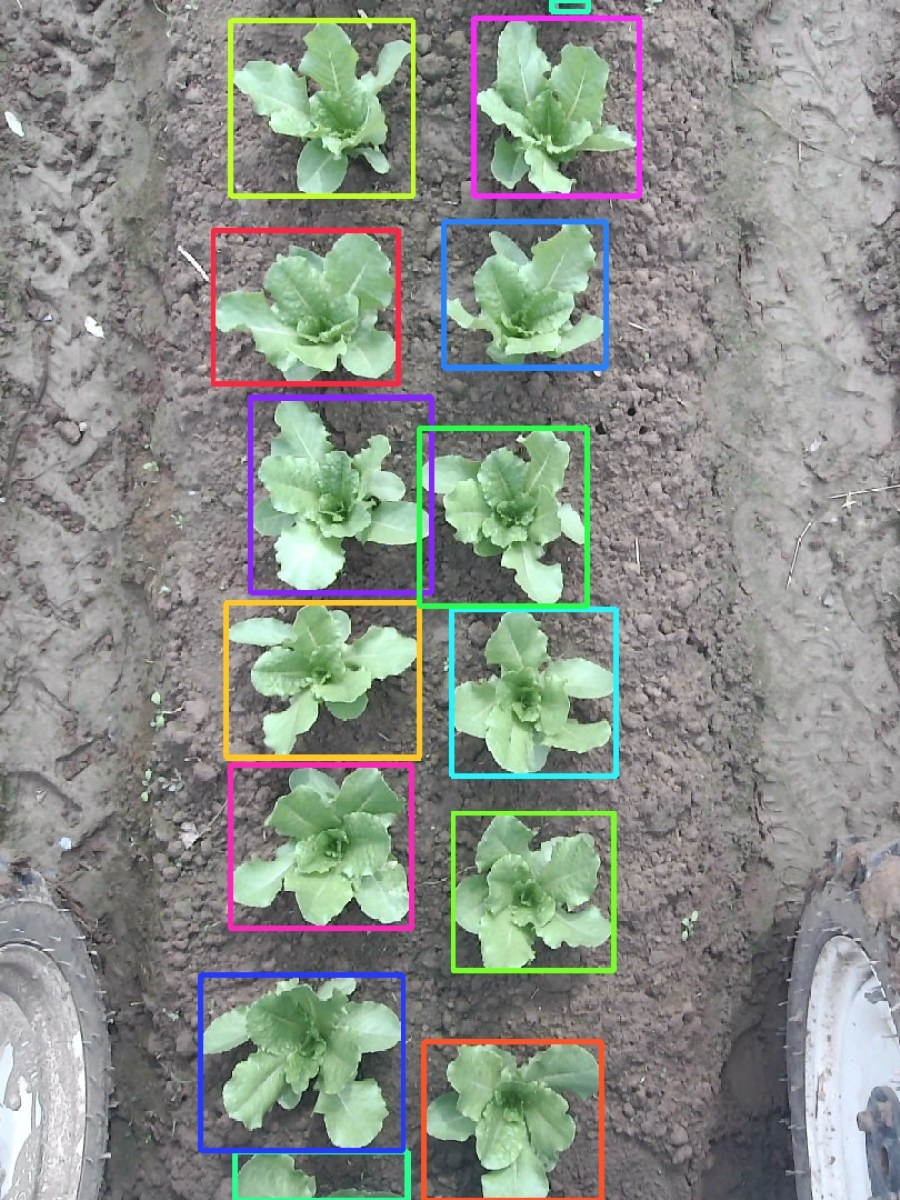
\includegraphics[height=0.165\textwidth]{figures/sample_lettuce.jpg} &
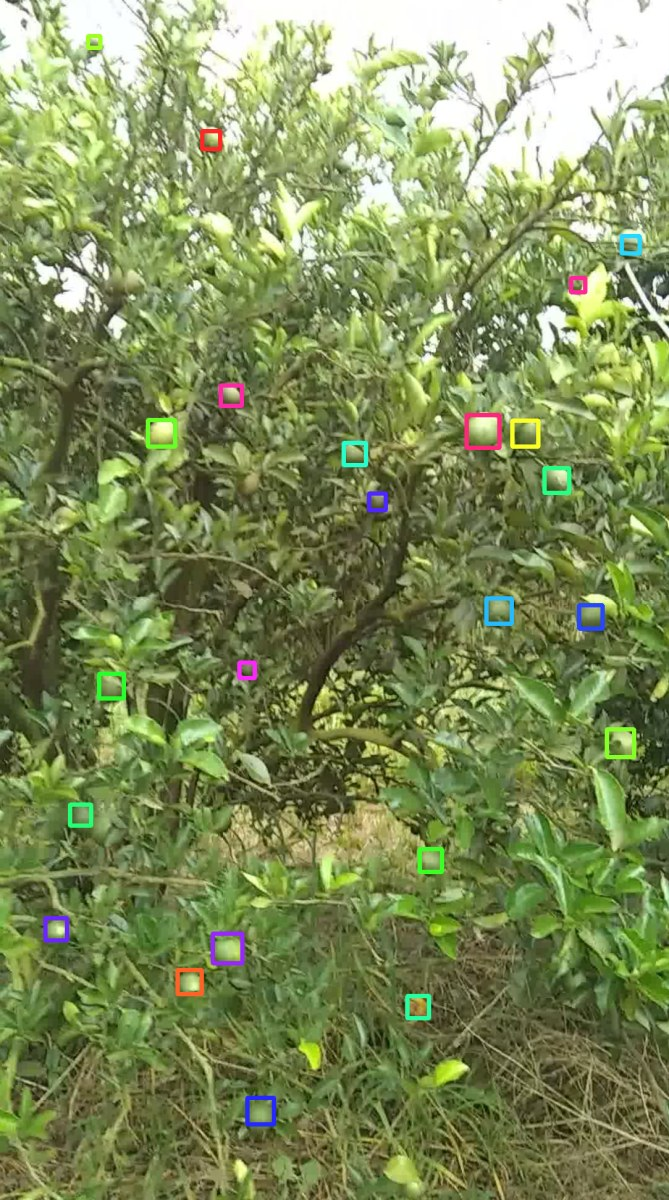
\includegraphics[height=0.165\textwidth]{figures/sample_orange.jpg} &
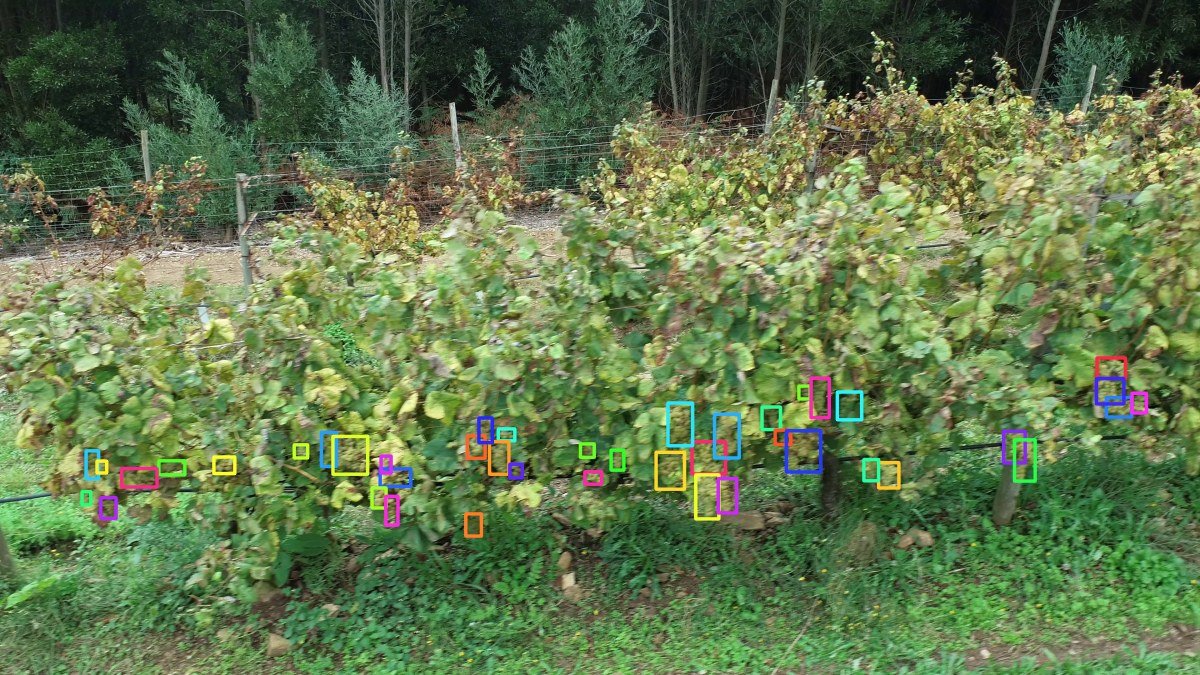
\includegraphics[height=0.165\textwidth]{figures/sample_grape.jpg} &
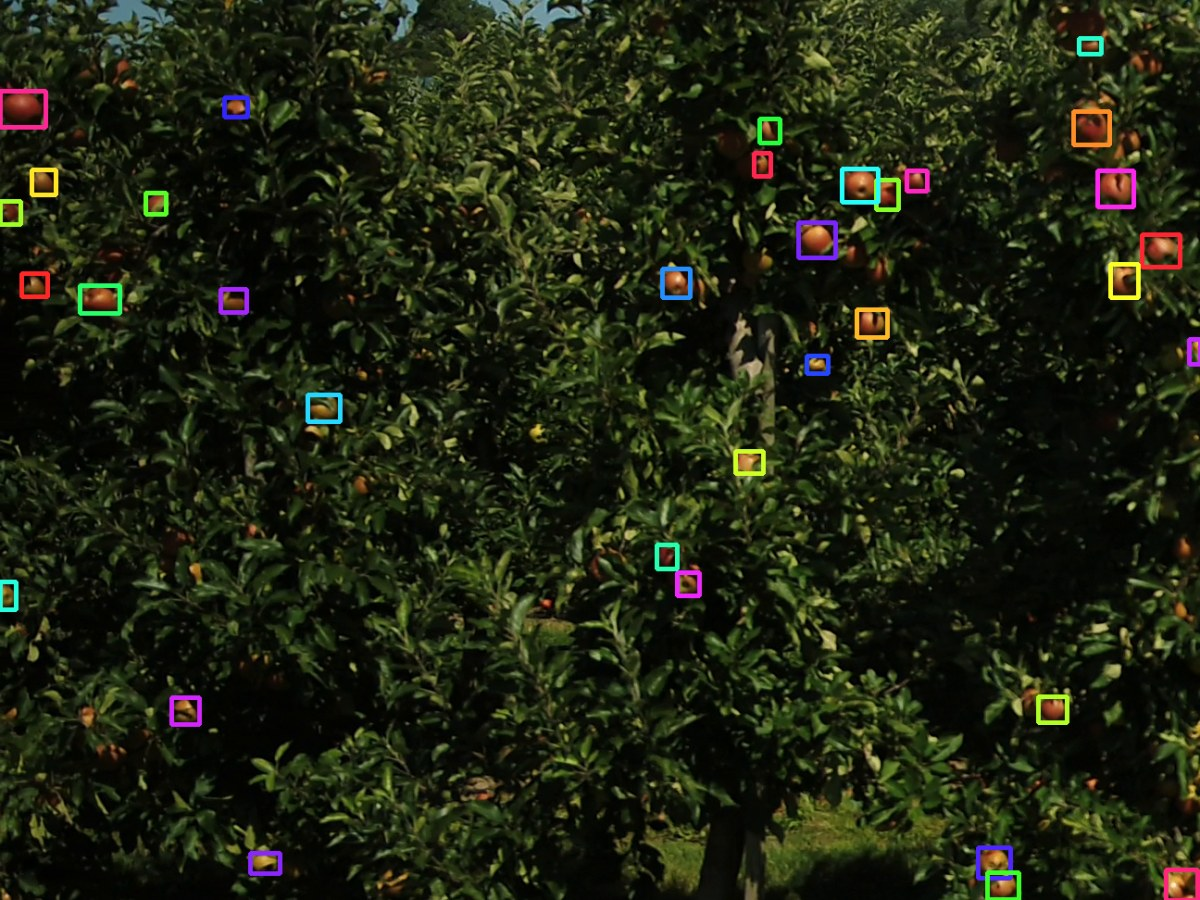
\includegraphics[height=0.165\textwidth]{figures/sample_apple.jpg} &
\figph{0.17\textwidth}{0.135\textwidth}{MangoYield\\sample frame} \\
{\scriptsize (a)} & {\scriptsize (b)} & {\scriptsize (c)} & {\scriptsize (d)} & {\scriptsize (e)}
\end{tabular}
\caption{Sample frames: (a) LettuceMOTS 0011, (b) MOrangeT V01, (c) GrapeMOTS PathPlanning\_7, (d) AppleMOTS 0008, with ground-truth boxes, and (e) MangoYield.}
\label{fig:samples}
\end{figure}

\subsection{Detections}\label{sec:detections}

Every tracker receives the same detections, produced by a YOLO detector \citep{jocher2023yolo} fine-tuned separately for each dataset. The detector is YOLO\tbd{} at an input size of \tbd{}\,px, initialised from COCO weights and fine-tuned on \tbd{}. Detections with a confidence above \tbd{} are passed to the trackers. On the evaluation sequences the detectors reach an AP$_{50}$ of \tbd{} on LettuceMOTS, \tbd{} on MOrangeT, \tbd{} on GrapeMOTS and \tbd{} on AppleMOTS.

\subsection{Baselines}\label{sec:baselines}

MapSORT is compared with BoT-SORT \citep{aharon2022botsort}, SAM2MOT \citep{jiang2025sam2mot} and StrongSORT \citep{du2023strongsort}, which together represent the strongest current approaches to the problem: fused motion and appearance association with camera-motion compensation, segmentation-propagation tracking, and cascaded appearance and motion association. All three are run from BoxMOT \citep{brostrom2024boxmot} with their default configurations and with the same detections as MapSORT. The appearance-based trackers share one re-identification model per dataset: OSNet-x0.25 \citep{zhou2019osnet}, initialised from MSMT17 and fine-tuned on object identities from \tbd{}. StrongSORT is also MapSORT's base tracker and shares all of its non-landmark hyperparameters, so comparing the two isolates the effect of the landmark cue.

\subsection{Evaluation metrics}\label{sec:metrics}

Tracking accuracy is measured with HOTA and its detection and association components DetA and AssA \citep{luiten2021hota}, MOTA and identity switches (IDSW) from the CLEAR metrics \citep{bernardin2008clear}, and IDF1 \citep{ristani2016idf1}, all computed with TrackEval \citep{luiten2020trackeval} at an IoU threshold of 0.5 for CLEAR and Identity. Two further metrics address the requirements of agricultural use.

\paragraph{Count error.} Yield estimation from video counts tracks. The count error
\begin{equation}
\mathrm{CE}=100\cdot\frac{|\mathrm{IDs}_{\text{pred}}|-|\mathrm{IDs}_{\text{GT}}|}{|\mathrm{IDs}_{\text{GT}}|}
\end{equation}
is the relative over-count (positive) or under-count (negative) of distinct identities; every identity switch that issues a new identity adds to it. On MangoYield, $|\mathrm{IDs}_{\text{pred}}|$ is the number of fruit identities a tracker issues over a tree's flight and $|\mathrm{IDs}_{\text{GT}}|$ is the tree's ground-truth yield count.

\paragraph{Revisit identity preservation.} A revisit event is a ground-truth object that reappears after at least $G=10$ consecutive frames out of view. At each event, the object's tracker identity is read, using exactly the per-frame assignment that CLEAR makes, at the first frame within a grace window of $W=5$ frames in which it is matched; the grace window allows for track confirmation after reappearance. The event is \emph{preserved} if that identity equals the one the object carried before the absence, a \emph{switch} if it differs, and \emph{unmatched} if the object is not matched within the window. The revisit identity preservation rate is
\begin{equation}
\RIP = 100\cdot\frac{\#\text{preserved}}{\#\text{preserved}+\#\text{switch}}.
\end{equation}
Because the per-frame assignment is CLEAR's own, every revisit switch is one of CLEAR's IDSW, so RIP measures the share of the hardest identity decisions, those after an absence, that a tracker gets right. Revisit outcomes are also reported as a function of absence length (Sect.~\ref{sec:res-revisit}).

\subsection{Implementation details}\label{sec:impl}

Table~\ref{tab:hparams} lists MapSORT's settings, which are identical across datasets except for the landmark point filters. The appearance and motion stages use StrongSORT's settings unchanged. Experiments ran on two machines: a laptop with an Intel Core i9-14900HX CPU and an NVIDIA GeForce RTX~4070 Laptop GPU (8\,GB), and, for the high-resolution GrapeMOTS and AppleMOTS sequences, a workstation with an Intel Xeon E3-1240~v5 CPU (4 cores, 8 threads, 3.5\,GHz) and no GPU.

\begin{table}[t]
\caption{MapSORT settings.}\label{tab:hparams}
\footnotesize
\begin{tabular*}{\textwidth}{@{\extracolsep\fill}lll@{}}
\toprule
Component & Parameter & Value \\
\midrule
\multirow{3}{*}{Detection} & Detector & YOLO\tbd, fine-tuned per dataset \\
 & Input size & \tbd \\
 & Confidence threshold & \tbd \\
\midrule
\multirow{3}{*}{Scene map} & SfM & COLMAP 3.9.1, shared RADIAL camera \\
 & Features & SIFT, $\le$16\,384 per frame, max.\ side 3840\,px \\
 & Matching & Exhaustive \\
\midrule
\multirow{5}{*}{Landmark filters} & LettuceMOTS & Excess green $\gamma=0.02$ \\
 & MOrangeT & Track length $\ell_{\min}=5$ \\
 & GrapeMOTS & None \\
 & AppleMOTS & \tbd \\
 & MangoYield & \tbd \\
\midrule
\multirow{4}{*}{Appearance} & Re-ID model & OSNet-x0.25, fine-tuned per dataset \\
 & Max.\ cosine distance & 0.4 \\
 & Gallery budget, EMA $\alpha$ & 100, 0.9 \\
 & Appearance weight $\lambda$ & 0.98 \\
\midrule
\multirow{3}{*}{Track management} & Confirmation $n_{\text{init}}$ & 3 \\
 & Max.\ age $A_{\max}$ & 30 frames \\
 & Max.\ IoU distance & 0.7 \\
\midrule
\multirow{2}{*}{Landmark association} & Gate $\tau$ & 200 \\
 & Dormant pool size & Unbounded \\
\midrule
\multirow{3}{*}{Evaluation} & IoU threshold & 0.5 \\
 & Revisit gap $G$, grace $W$ & 10, 5 frames \\
 & Toolkit & TrackEval 1.3.0 \\
\botrule
\end{tabular*}
\end{table}

%% =====================================================================
\section{Results}\label{sec:results}

\subsection{Comparison with state-of-the-art trackers}\label{sec:res-main}

Table~\ref{tab:main} compares MapSORT with the three baselines on all four datasets. MapSORT achieves the highest HOTA, AssA and IDF1 on every dataset. % TODO confirm once all runs are complete
The gains concentrate in association: DetA, which reflects localisation and is shared by all trackers given the same detections, moves little, while AssA rises by \tbd{} points on average over the strongest baseline. On the datasets with revisits, MapSORT preserves identity in \tbd{}\% of revisit events, against \tbd{}\% for the best baseline. Count error falls from \tbd{}\% to \tbd{}\% on average, which translates directly into more accurate yield estimates. On AppleMOTS, where objects are never out of view for long, the landmark stage still improves association among dense clusters of near-identical apples (HOTA \tbd{} vs.\ \tbd{}).

\begin{table}[t]
\caption{Tracking results. CE: count error (\%). RIP: revisit identity preservation rate (\%); AppleMOTS has no revisit events. Best per dataset in bold.}\label{tab:main}
\footnotesize
\setlength{\tabcolsep}{3.5pt}
\begin{tabular*}{\textwidth}{@{\extracolsep\fill}llrrrrrrrr@{}}
\toprule
Dataset & Tracker & HOTA$\uparrow$ & AssA$\uparrow$ & DetA$\uparrow$ & MOTA$\uparrow$ & IDF1$\uparrow$ & IDSW$\downarrow$ & CE$\downarrow$ & RIP$\uparrow$ \\
\midrule
\multirow{4}{*}{LettuceMOTS} & BoT-SORT & \tbd & \tbd & \tbd & \tbd & \tbd & \tbd & \tbd & \tbd \\
 & SAM2MOT & \tbd & \tbd & \tbd & \tbd & \tbd & \tbd & \tbd & \tbd \\
 & StrongSORT & 69.97 & 52.90 & 92.54 & 90.82 & 57.41 & 167 & +107.0 & 2.9 \\
 & MapSORT & \tbd & \tbd & \tbd & \tbd & \tbd & \tbd & \tbd & \tbd \\
\midrule
\multirow{4}{*}{MOrangeT} & BoT-SORT & \tbd & \tbd & \tbd & \tbd & \tbd & \tbd & \tbd & \tbd \\
 & SAM2MOT & \tbd & \tbd & \tbd & \tbd & \tbd & \tbd & \tbd & \tbd \\
 & StrongSORT & \tbd & \tbd & \tbd & \tbd & \tbd & \tbd & \tbd & \tbd \\
 & MapSORT & \tbd & \tbd & \tbd & \tbd & \tbd & \tbd & \tbd & \tbd \\
\midrule
\multirow{4}{*}{GrapeMOTS} & BoT-SORT & \tbd & \tbd & \tbd & \tbd & \tbd & \tbd & \tbd & \tbd \\
 & SAM2MOT & \tbd & \tbd & \tbd & \tbd & \tbd & \tbd & \tbd & \tbd \\
 & StrongSORT & \tbd & \tbd & \tbd & \tbd & \tbd & \tbd & \tbd & \tbd \\
 & MapSORT & \tbd & \tbd & \tbd & \tbd & \tbd & \tbd & \tbd & \tbd \\
\midrule
\multirow{4}{*}{AppleMOTS} & BoT-SORT & \tbd & \tbd & \tbd & \tbd & \tbd & \tbd & \tbd & n/a \\
 & SAM2MOT & \tbd & \tbd & \tbd & \tbd & \tbd & \tbd & \tbd & n/a \\
 & StrongSORT & \tbd & \tbd & \tbd & \tbd & \tbd & \tbd & \tbd & n/a \\
 & MapSORT & \tbd & \tbd & \tbd & \tbd & \tbd & \tbd & \tbd & n/a \\
\botrule
\end{tabular*}
\end{table}

\subsection{Representative sequences}\label{sec:res-seq}

One representative sequence per dataset is used for the detailed analyses that follow: LettuceMOTS 0011, MOrangeT V01, GrapeMOTS PathPlanning\_7 and AppleMOTS 0008. Table~\ref{tab:seq} reports all trackers on these sequences.

On LettuceMOTS 0011 the robot drives out along two rows and returns, so each of the 37 plants is seen twice. StrongSORT issues 60 identities and switches identity at every one of the 22 revisit events. MapSORT tracks all 37 plants with a single identity each: zero identity switches, all 22 revisits preserved, IDF1 98.0 and HOTA 96.2, an improvement of 19.9 HOTA and 34.0 IDF1 points. The plant count is exact.

On MOrangeT V01, a handheld sweep around an orange tree with 104 revisit events, MapSORT raises HOTA from 71.4 to 87.1 and IDF1 from 62.8 to 84.6, more than halves identity switches (129 to 70), and preserves identity in 69.0\% of revisits against 15.8\%. The count error falls from +101.8\% to +41.8\%. This holds although the oranges' landmarks rest on few points (a median of two per detection, Table~\ref{tab:recon}), which shows that the fused landmark accumulates usable precision from sparse support.

On GrapeMOTS PathPlanning\_7, where the UAV views the vines from several perspectives, MapSORT raises HOTA from 78.1 to 92.3 and IDF1 from 72.9 to 92.2, halves identity switches (125 to 56), and reduces count error from +123.1\% to +41.5\%. StrongSORT preserves none of the 23 revisits; MapSORT preserves 8.

\begin{table}[t]
\caption{Results on the representative sequences. Columns as in Table~\ref{tab:main}. AppleMOTS 0008 has no revisit events.}\label{tab:seq}
\footnotesize
\setlength{\tabcolsep}{3.5pt}
\begin{tabular*}{\textwidth}{@{\extracolsep\fill}llrrrrrrrr@{}}
\toprule
Sequence & Tracker & HOTA$\uparrow$ & AssA$\uparrow$ & DetA$\uparrow$ & MOTA$\uparrow$ & IDF1$\uparrow$ & IDSW$\downarrow$ & CE$\downarrow$ & RIP$\uparrow$ \\
\midrule
\multirow{4}{*}{\shortstack[l]{LettuceMOTS\\0011}} & BoT-SORT & \tbd & \tbd & \tbd & \tbd & \tbd & \tbd & \tbd & \tbd \\
 & SAM2MOT & \tbd & \tbd & \tbd & \tbd & \tbd & \tbd & \tbd & \tbd \\
 & StrongSORT & 76.33 & 62.17 & 93.72 & 92.97 & 64.03 & 23 & +62.2 & 0.0 \\
 & MapSORT & \textbf{96.20} & \textbf{96.24} & \textbf{96.16} & \textbf{96.16} & \textbf{98.04} & \textbf{0} & \textbf{0.0} & \textbf{100.0} \\
\midrule
\multirow{4}{*}{\shortstack[l]{MOrangeT\\V01}} & BoT-SORT & \tbd & \tbd & \tbd & \tbd & \tbd & \tbd & \tbd & \tbd \\
 & SAM2MOT & \tbd & \tbd & \tbd & \tbd & \tbd & \tbd & \tbd & \tbd \\
 & StrongSORT & 71.35 & 54.42 & 93.57 & 91.92 & 62.77 & 129 & +101.8 & 15.8 \\
 & MapSORT & \textbf{87.13} & \textbf{79.61} & \textbf{95.36} & \textbf{94.47} & \textbf{84.56} & \textbf{70} & \textbf{+41.8} & \textbf{69.0} \\
\midrule
\multirow{4}{*}{\shortstack[l]{GrapeMOTS\\PathPlanning\_7}} & BoT-SORT & \tbd & \tbd & \tbd & \tbd & \tbd & \tbd & \tbd & \tbd \\
 & SAM2MOT & \tbd & \tbd & \tbd & \tbd & \tbd & \tbd & \tbd & \tbd \\
 & StrongSORT & 78.12 & 63.43 & 96.22 & 94.95 & 72.90 & 125 & +123.1 & 0.0 \\
 & MapSORT & \textbf{92.25} & \textbf{87.39} & \textbf{97.39} & \textbf{97.15} & \textbf{92.21} & \textbf{56} & \textbf{+41.5} & \textbf{34.8} \\
\midrule
\multirow{4}{*}{\shortstack[l]{AppleMOTS\\0008}} & BoT-SORT & \tbd & \tbd & \tbd & \tbd & \tbd & \tbd & \tbd & n/a \\
 & SAM2MOT & \tbd & \tbd & \tbd & \tbd & \tbd & \tbd & \tbd & n/a \\
 & StrongSORT & \tbd & \tbd & \tbd & \tbd & \tbd & \tbd & \tbd & n/a \\
 & MapSORT & \tbd & \tbd & \tbd & \tbd & \tbd & \tbd & \tbd & n/a \\
\botrule
\end{tabular*}
\end{table}

\subsection{Identity persistence across revisits}\label{sec:res-revisit}

Fig.~\ref{fig:gap} breaks revisit outcomes down by how long the object was out of view. StrongSORT preserves identity only for short absences: 62.5\% of events with a gap below 30 frames, and none at all beyond, because a track unmatched for $A_{\max}=30$ frames is deleted. MapSORT preserves identity across every absence length, at 54.8\% to 84.6\% per bin, and its preservation rate does not decline with gap length: it is 72.3\% for absences of 120 frames or more. This is the behaviour Sect.~\ref{sec:dormant} is designed to produce: the landmark of a stationary object does not age, so a dormant track is as recoverable after a long absence as after a short one.

\begin{figure}[t]
\centering
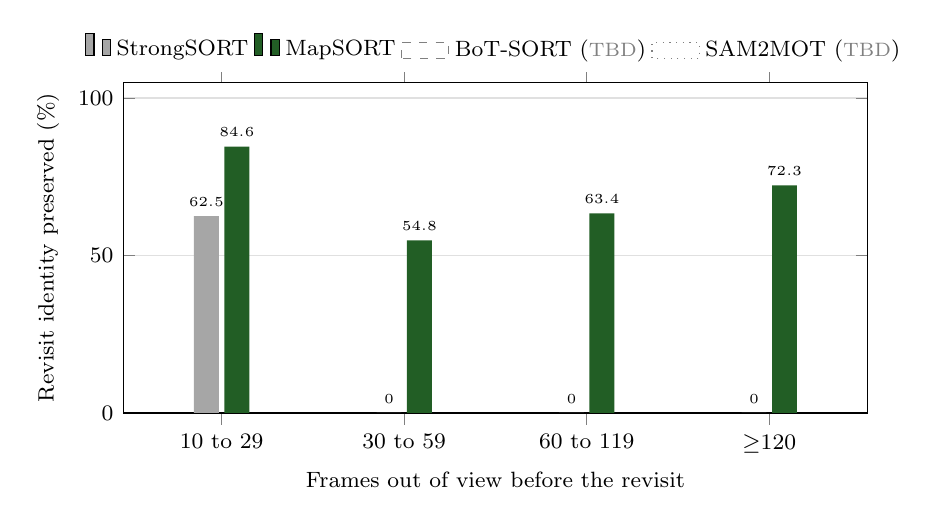
\begin{tikzpicture}
\begin{axis}[
  ybar, bar width=9pt, scale only axis, width=0.78\textwidth, height=4.2cm,
  ymin=0, ymax=105, ylabel={Revisit identity preserved (\%)},
  xlabel={Frames out of view before the revisit},
  symbolic x coords={10 to 29,30 to 59,60 to 119,$\geq$120}, xtick=data,
  enlarge x limits=0.18,
  legend style={at={(0.5,1.03)}, anchor=south, legend columns=4, draw=none, font=\footnotesize},
  nodes near coords, nodes near coords style={font=\tiny, /pgf/number format/fixed, /pgf/number format/precision=1},
  every axis plot/.append style={draw=none},
  tick label style={font=\footnotesize}, label style={font=\footnotesize},
  ymajorgrids, grid style={black!12},
]
% StrongSORT and MapSORT: LettuceMOTS 0011, MOrangeT V01, GrapeMOTS PathPlanning_7 pooled (149 events).
% TODO add BoT-SORT and SAM2MOT, and pool all revisit sequences once runs complete.
\addplot[fill=black!35] coordinates {(10 to 29,62.5) (30 to 59,0.0) (60 to 119,0.0) ($\geq$120,0.0)};
\addplot[fill=clm!75!black] coordinates {(10 to 29,84.6) (30 to 59,54.8) (60 to 119,63.4) ($\geq$120,72.3)};
\addlegendentry{StrongSORT}
\addlegendentry{MapSORT}
\addlegendimage{area legend, draw=black!50, dashed, fill=white}\addlegendentry{BoT-SORT (\tbd)}
\addlegendimage{area legend, draw=black!50, dotted, fill=white}\addlegendentry{SAM2MOT (\tbd)}
\end{axis}
\end{tikzpicture}
\caption{Revisit identity preservation by length of absence, over the 149 revisit events of the representative sequences. StrongSORT deletes tracks unseen for more than 30 frames and preserves no identity beyond that horizon; MapSORT's dormant tracks keep identities recoverable at every absence length.}
\label{fig:gap}
\end{figure}

\subsection{Yield estimation in a mango orchard}\label{sec:res-yield}

Table~\ref{tab:yield} compares each tracker's fruit count with the yield count of the three MangoYield trees. An orbit around a tree is a demanding case for counting: every fruit on the near side is seen again from the far side as the orbit closes, and a tracker that forgets it counts it twice. MapSORT's count is within \tbd{}\% of the ground truth on average, against \tbd{}\% for the best baseline, because a fruit seen from the far side of the tree occupies the same position in the scene map as when it was first seen.

\begin{table}[t]
\caption{Fruit counts on MangoYield. Each cell gives the number of fruit identities issued over the tree's flight, with the count error CE (\%) in parentheses. Mean $|$CE$|$ is averaged over the three trees.}\label{tab:yield}
\footnotesize
\begin{tabular*}{\textwidth}{@{\extracolsep\fill}lrrrrr@{}}
\toprule
Tree & GT count & BoT-SORT & SAM2MOT & StrongSORT & MapSORT \\
\midrule
Tree 1 & \tbd & \tbd{} (\tbd) & \tbd{} (\tbd) & \tbd{} (\tbd) & \tbd{} (\tbd) \\
Tree 2 & \tbd & \tbd{} (\tbd) & \tbd{} (\tbd) & \tbd{} (\tbd) & \tbd{} (\tbd) \\
Tree 3 & \tbd & \tbd{} (\tbd) & \tbd{} (\tbd) & \tbd{} (\tbd) & \tbd{} (\tbd) \\
\midrule
Mean $|$CE$|$ (\%) & & \tbd & \tbd & \tbd & \tbd \\
\botrule
\end{tabular*}
\end{table}

\subsection{Ablation study}\label{sec:res-ablation}

Table~\ref{tab:ablation} isolates each component on the representative sequences, building from StrongSORT (a) to the full MapSORT (c). Adding landmark association to the active tracks (b) recovers objects that the appearance cascade misses while their tracks are still alive; adding dormant revival (c) extends recovery beyond the deletion horizon and accounts for the gains at long absences in Fig.~\ref{fig:gap}. Together they raise pooled revisit preservation from 10.7\% to 68.3\%. Removing the appearance stage (d) shows how much of MapSORT's association the landmark alone carries. Replacing the Gaussian landmark by the nearest triangulated keypoint to the box centre with a Euclidean gate (e), the point-estimate localisation of prior fruit-tracking work, quantifies the contribution of the uncertainty-aware observation model and of scale-invariant gating.

\begin{table}[t]
\caption{Ablation on the representative sequences (HOTA / IDF1). RIP is pooled over the revisit events of all four sequences. (e) uses the nearest SfM keypoint to the box centre as a point landmark with a Euclidean distance gate.}\label{tab:ablation}
\scriptsize
\setlength{\tabcolsep}{1.6pt}
\begin{tabular*}{\textwidth}{@{\extracolsep\fill}lrrrrrrrrr@{}}
\toprule
 & \multicolumn{2}{c}{Lettuce 0011} & \multicolumn{2}{c}{Orange V01} & \multicolumn{2}{c}{Grape PP\_7} & \multicolumn{2}{c}{Apple 0008} & \\
\cmidrule(lr){2-3}\cmidrule(lr){4-5}\cmidrule(lr){6-7}\cmidrule(lr){8-9}
Variant & HOTA & IDF1 & HOTA & IDF1 & HOTA & IDF1 & HOTA & IDF1 & RIP \\
\midrule
(a) StrongSORT & 76.33 & 64.03 & 71.35 & 62.77 & 78.12 & 72.90 & \tbd & \tbd & 10.7 \\
(b) + landmark assoc. & \tbd & \tbd & \tbd & \tbd & \tbd & \tbd & \tbd & \tbd & \tbd \\
(c) + dormancy (MapSORT) & \textbf{96.20} & \textbf{98.04} & \textbf{87.13} & \textbf{84.56} & \textbf{92.25} & \textbf{92.21} & \tbd & \tbd & \textbf{68.3} \\
(d) (c) w/o appearance & \tbd & \tbd & \tbd & \tbd & \tbd & \tbd & \tbd & \tbd & \tbd \\
(e) (c), point landmark & \tbd & \tbd & \tbd & \tbd & \tbd & \tbd & \tbd & \tbd & \tbd \\
\botrule
\end{tabular*}
\end{table}

\subsection{Sensitivity to the landmark gate}\label{sec:res-gate}

Fig.~\ref{fig:gate} sweeps the landmark gate $\tau$ over two orders of magnitude, from the 95\% quantile of the $\chi^2_3$ distribution (7.81) to 1600. Because the gating distance is invariant to reconstruction scale (Proposition~\ref{prop:scale}), a single value serves all four datasets. HOTA and revisit preservation are stable over a broad range around the default $\tau=200$. % TODO describe the curve once the sweep is run

\begin{figure}[t]
\centering

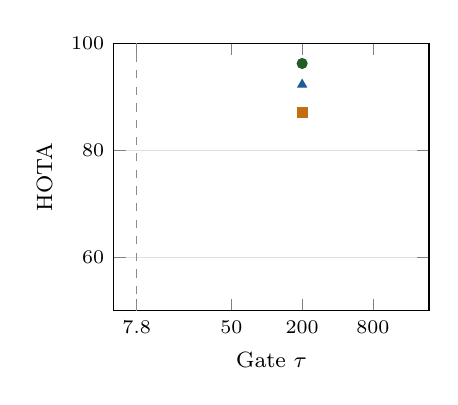
\begin{tikzpicture}
\begin{axis}[
  scale only axis, width=0.33\textwidth, height=3.4cm, xmode=log, log basis x=10,
  xmin=5, xmax=2400, xtick={7.81,50,200,800},
  xticklabels={7.8,50,200,800}, xlabel={Gate $\tau$},
  tick label style={font=\scriptsize}, label style={font=\footnotesize},
  ymajorgrids, grid style={black!12}, mark size=1.8pt, ymin=50, ymax=100, ylabel={HOTA},
  legend to name=gatelegend, legend columns=4, legend style={draw=none, font=\scriptsize, /tikz/every even column/.append style={column sep=6pt}}]
\draw[dashed, black!45] (axis cs:7.81,50) -- (axis cs:7.81,100);
% TODO fill the sweep; each series is one representative sequence
\addplot[clm!75!black, mark=*] coordinates {(200,96.20)};
\addplot[capp, mark=square*] coordinates {(200,87.13)};
\addplot[cmap, mark=triangle*] coordinates {(200,92.25)};
\addlegendimage{black!60, mark=diamond*}
\legend{Lettuce 0011, Orange V01, Grape PP\_7, Apple 0008 (\tbd)}
\end{axis}
\end{tikzpicture}\hfill
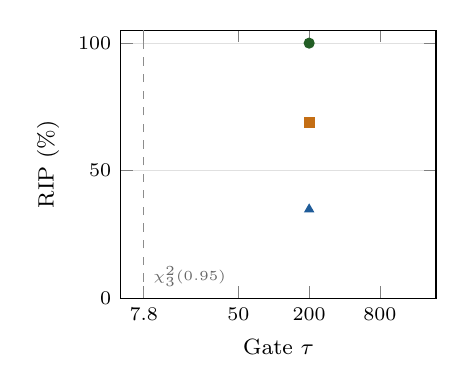
\begin{tikzpicture}
\begin{axis}[
  scale only axis, width=0.33\textwidth, height=3.4cm, xmode=log, log basis x=10,
  xmin=5, xmax=2400, xtick={7.81,50,200,800},
  xticklabels={7.8,50,200,800}, xlabel={Gate $\tau$},
  tick label style={font=\scriptsize}, label style={font=\footnotesize},
  ymajorgrids, grid style={black!12}, mark size=1.8pt, ymin=0, ymax=105, ylabel={RIP (\%)}]
\draw[dashed, black!45] (axis cs:7.81,0) -- (axis cs:7.81,105) node[pos=0.08, right, font=\tiny, black!60] {$\chi^2_3(0.95)$};
\addplot[clm!75!black, mark=*] coordinates {(200,100.0)};
\addplot[capp, mark=square*] coordinates {(200,69.0)};
\addplot[cmap, mark=triangle*] coordinates {(200,34.8)};
\end{axis}
\end{tikzpicture}\\[2pt]
\pgfplotslegendfromname{gatelegend}
\caption{Sensitivity of HOTA (left) and revisit identity preservation (right) to the landmark gate $\tau$ on the representative sequences. The dashed line marks the $\chi^2_3$ 95\% quantile. AppleMOTS 0008 has no revisit events and appears only on the left.}
\label{fig:gate}
\end{figure}

\subsection{Scene maps and runtime}\label{sec:res-runtime}

COLMAP registers every frame of every representative sequence into a single model (Table~\ref{tab:recon}), with sub-pixel to about one-pixel mean reprojection error. Most detections receive a landmark: 98.6\% on LettuceMOTS, 93.3\% on GrapeMOTS and 76.9\% on MOrangeT, where small, glossy fruit seen against foliage yield fewer stable keypoints. Fig.~\ref{fig:recon} shows the reconstruction of LettuceMOTS 0011: the two rows of plants and the camera path along them, with the outbound and return passes registered into the same map.

\begin{table}[t]
\caption{Scene maps on the representative sequences. Track len.: mean number of frames observing a 3D point. Cov.: share of detections that receive a landmark. Pts/LM: median number of map points supporting a landmark observation.}\label{tab:recon}
\footnotesize
\setlength{\tabcolsep}{2.5pt}
\begin{tabular*}{\textwidth}{@{\extracolsep\fill}lrrrrrrr@{}}
\toprule
Sequence & Reg.\ frames & 3D points & Track len. & Reproj.\ (px) & Cov.\ (\%) & Pts/LM & SfM (min) \\
\midrule
LettuceMOTS 0011 & 223/223 & 168\,466 & 17.7 & 0.73 & 98.6 & 162 & \tbd \\
MOrangeT V01 & 408/408 & 69\,081 & 10.0 & 1.16 & 76.9 & 2 & \tbd \\
GrapeMOTS PP\_7 & 225/225 & 129\,210 & 19.1 & 0.96 & 93.3 & 13 & \tbd \\
AppleMOTS 0008 & \tbd & \tbd & \tbd & \tbd & \tbd & \tbd & \tbd \\
\botrule
\end{tabular*}
\end{table}

\begin{figure}[t]
\centering
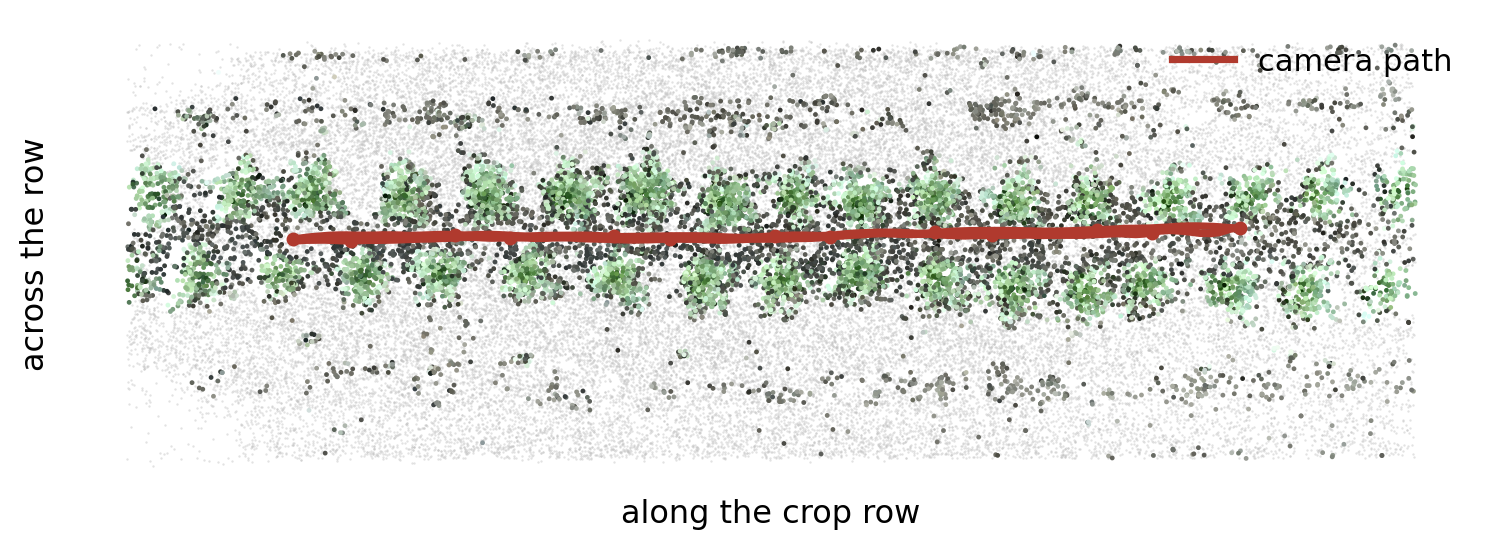
\includegraphics[width=0.9\textwidth]{figures/reconstruction.png}
\caption{Sparse scene map of LettuceMOTS 0011, viewed from above. Plant points are green, soil grey; the line is the reconstructed camera path. The outbound and return passes are registered into one map, so each plant has one position on both.}
\label{fig:recon}
\end{figure}

Table~\ref{tab:runtime} reports tracking throughput. MapSORT runs at the same throughput as StrongSORT on MOrangeT and GrapeMOTS, and at about 80\% of it on LettuceMOTS: landmark association and fusion operate on $3\times3$ matrices and add little to a frame's cost, which is dominated by appearance embedding. The map is built once per sequence, before tracking.

\begin{table}[t]
\caption{Tracking throughput (frames per second, including image decoding, detection and appearance embedding; excluding map construction). Hardware: L, laptop with RTX~4070 Laptop GPU; W, CPU-only workstation (Sect.~\ref{sec:impl}).}\label{tab:runtime}
\footnotesize
\begin{tabular*}{\textwidth}{@{\extracolsep\fill}lcrrrr@{}}
\toprule
Sequence & Hardware & BoT-SORT & SAM2MOT & StrongSORT & MapSORT \\
\midrule
LettuceMOTS 0011 & L & \tbd & \tbd & 5.05 & 4.03 \\
MOrangeT V01 & L & \tbd & \tbd & 1.70 & 1.72 \\
GrapeMOTS PP\_7 & W & \tbd & \tbd & 0.70 & 0.70 \\
AppleMOTS 0008 & W & \tbd & \tbd & \tbd & \tbd \\
\botrule
\end{tabular*}
\end{table}

\subsection{Qualitative results}\label{sec:res-qual}

Fig.~\ref{fig:qual} compares StrongSORT and MapSORT on the return pass of LettuceMOTS 0011. By this frame StrongSORT has issued 50 identities for 37 plants: every plant on screen carries a new identity, assigned when it reappeared. MapSORT shows each plant with the identity it received on the outbound pass and has issued exactly 37 identities. Fig.~\ref{fig:qual-other} shows the corresponding comparison on the other datasets.

\begin{figure}[t]
\centering
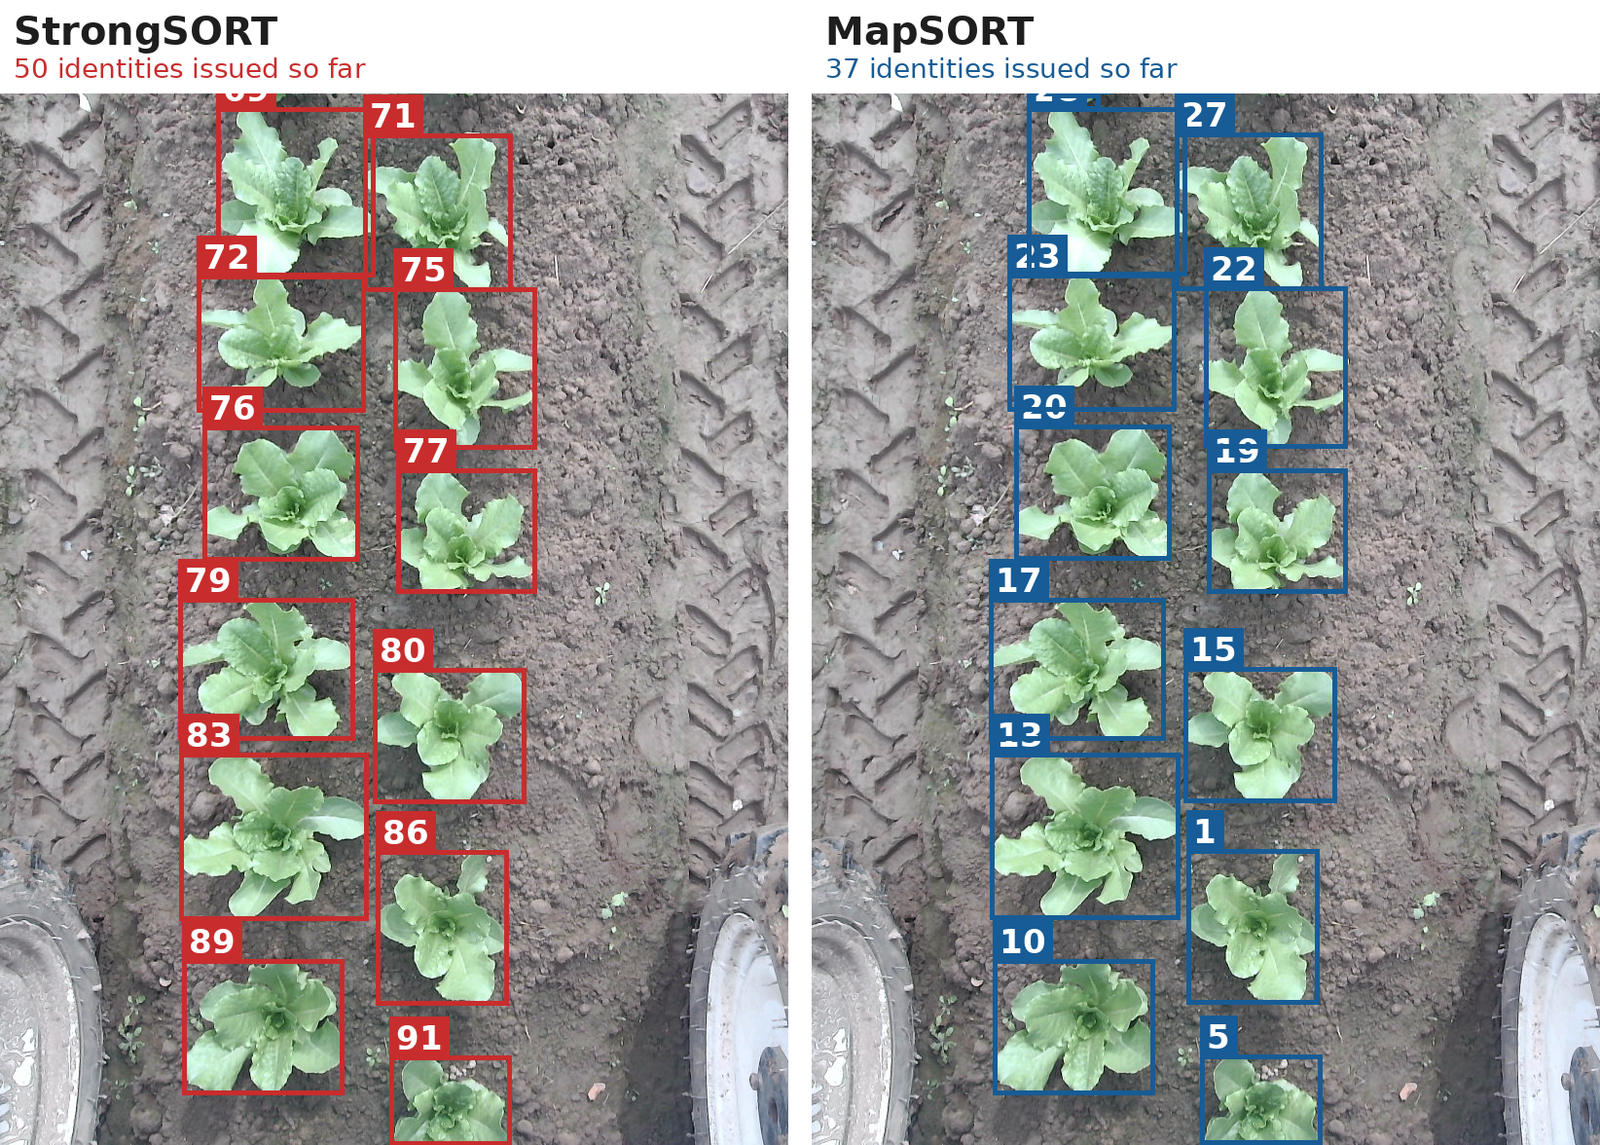
\includegraphics[width=0.8\textwidth]{figures/strongsort_vs_mapsort.png}
\caption{Return pass of LettuceMOTS 0011. Left: StrongSORT has issued 50 identities so far and labels every returning plant with a new one. Right: MapSORT restores each plant's outbound identity and has issued 37 identities, one per plant.}
\label{fig:qual}
\end{figure}

\begin{figure}[t]
\centering
\figph{0.3\textwidth}{3.4cm}{MOrangeT V01:\\StrongSORT vs.\ MapSORT\\at a fruit re-entry}\hfill
\figph{0.3\textwidth}{3.4cm}{GrapeMOTS PP\_7:\\StrongSORT vs.\ MapSORT\\after a perspective change}\hfill
\figph{0.3\textwidth}{3.4cm}{AppleMOTS 0008:\\StrongSORT vs.\ MapSORT\\in a dense cluster}
\caption{Qualitative comparison on (a) MOrangeT V01, (b) GrapeMOTS PathPlanning\_7 and (c) AppleMOTS 0008.}
\label{fig:qual-other}
\end{figure}

%% =====================================================================
\section{Discussion}\label{sec:discussion}

The results show that, for stationary agricultural targets, a scene-map position is the identity cue that survives the conditions under which appearance and image-plane motion fail. The effect is largest exactly where agricultural tracking is hardest. When the camera returns to an object after a long absence, StrongSORT's identity is lost by construction, and MapSORT recovers it at a rate that does not decay with the length of the absence (Fig.~\ref{fig:gap}). On LettuceMOTS 0011, which is the operating pattern of a field robot working a row and returning, this turns a tracker that assigns two identities to every plant into one that assigns exactly one.

For precision agriculture, the most direct consequence is counting. Every identity switch that issues a new identity is a phantom plant or fruit in the count. StrongSORT over-counts by 62\% to 123\% on the representative sequences, which would make its output unusable as a yield estimate without heavy post-hoc correction. MapSORT's count is exact on LettuceMOTS 0011 and its over-count is roughly a third of StrongSORT's on MOrangeT and GrapeMOTS. A second consequence is per-plant records. Because a plant keeps its identity across passes, measurements taken on the outbound and return passes, or from different UAV perspectives, attach to the same plant, which is what plant-level phenotyping and selective treatment need. A third is spatial: every MapSORT track carries a position in the scene map, so a track list is also a plant map. Registering the map to a GNSS-referenced frame, as is routine in orchard and field mapping, would turn MapSORT's output into a georeferenced inventory of individual plants or fruit.

The landmark model generalises across very different acquisition conditions: a nadir camera over lettuce with dense map support, a handheld sweep of an orange canopy where landmarks rest on a median of two points, and high-resolution UAV video of a vineyard viewed from multiple perspectives. The same gate value serves all of them, a direct consequence of the scale invariance of the Mahalanobis gate (Proposition~\ref{prop:scale}); a metric distance threshold would have needed retuning for each reconstruction. MapSORT also composes with an existing tracker rather than replacing it. The appearance and motion stages are StrongSORT's, unchanged, and the landmark stages act on what they leave unmatched; any improvement in appearance models or detectors carries over to MapSORT directly.

%% =====================================================================
\section{Conclusion}\label{sec:conclusion}

MapSORT turns the stationarity of crops and fruit into an identity cue. It lifts each detection to a Gaussian landmark in a structure-from-motion map of the scene, fuses landmarks across a track's observations, associates them with a scale-invariant Mahalanobis gate inside a StrongSORT cascade, and revives dormant tracks by landmark when the camera returns. On four public agricultural datasets covering lettuce, oranges, grapes and apples, recorded from a field robot, a handheld camera, a wearable camera and a UAV, MapSORT outperforms BoT-SORT, SAM2MOT and StrongSORT, preserves identity across revisits of any length, and produces substantially more accurate counts, including per-tree yield counts in a mango orchard. MapSORT currently builds its scene map offline. Recent online reconstruction models that recover camera pose and scene geometry frame by frame from monocular video \citep{wang2025cut3r,murai2025mast3rslam} are a natural drop-in source for the same landmark observations, and extending MapSORT to online operation on a field robot is the subject of future work.

\backmatter

\bmhead{Acknowledgements}
\tbd

\section*{Statements and Declarations}

\bmhead{Funding}
\tbd

\bmhead{Competing interests}
The author has no relevant financial or non-financial interests to disclose.

\bmhead{Ethics approval and consent}
Not applicable.

\bmhead{Data availability}
All datasets used are publicly available from their original publishers: LettuceMOTS \citep{hu2024lettucemots}, MOrangeT \citep{santos2024moranget}, GrapeMOTS \citep{arizasentis2024grapemots} and AppleMOTS \citep{dejong2022applemots}. The MangoYield dataset collected for this work is available from the author on reasonable request. % TODO confirm availability terms

\bmhead{Code availability}
The MapSORT source code is available at \url{https://github.com/shinobi-wolf/MapSORT}. % TODO confirm the repository will be public at submission

\bmhead{Author contributions}
Srihari Vemuru conceived the method, implemented it, conducted the experiments and wrote the manuscript.

% TODO Springer policy: state any use of AI tools in preparing the manuscript, if applicable.

\clearpage
\begin{appendices}

\section{Per-sequence statistics}\label{sec:app-seq}

\begin{table}[!h]
\caption{Statistics of every evaluation sequence. MangoYield has one flight per tree and no per-frame annotations. Revisits: ground-truth objects reappearing after at least 10 frames out of view.}\label{tab:seqstats}
\footnotesize
\begin{tabular*}{\textwidth}{@{\extracolsep\fill}llrlrrr@{}}
\toprule
Dataset & Sequence & Frames & Resolution & GT IDs & Boxes & Revisits \\
\midrule
\multirow{3}{*}{LettuceMOTS} & 0003 & 245 & 810$\times$1080 & 40 & 3\,304 & 25 \\
 & 0007 & 244 & 810$\times$1080 & 37 & 3\,341 & 23 \\
 & 0011 & 223 & 810$\times$1080 & 37 & 3\,073 & 22 \\
\midrule
\multirow{12}{*}{MOrangeT} & V01 & 408 & 1083$\times$1944 & 110 & 7\,848 & 104 \\
 & V02 & \tbd & \tbd & \tbd & \tbd & \tbd \\
 & V03 & \tbd & \tbd & \tbd & \tbd & \tbd \\
 & V04 & \tbd & \tbd & \tbd & \tbd & \tbd \\
 & V05 & \tbd & \tbd & \tbd & \tbd & \tbd \\
 & V06 & \tbd & \tbd & \tbd & \tbd & \tbd \\
 & V07 & \tbd & \tbd & \tbd & \tbd & \tbd \\
 & V08 & \tbd & \tbd & \tbd & \tbd & \tbd \\
 & V09 & \tbd & \tbd & \tbd & \tbd & \tbd \\
 & V10 & \tbd & \tbd & \tbd & \tbd & \tbd \\
 & V11 & \tbd & \tbd & \tbd & \tbd & \tbd \\
 & V12 & \tbd & \tbd & \tbd & \tbd & \tbd \\
\midrule
\multirow{8}{*}{GrapeMOTS} & PathPlanning\_1 & 927 & 1920$\times$1080 & 29 & 4\,796 & 0 \\
 & PathPlanning\_2 & 209 & 3840$\times$2160 & 45 & 4\,838 & 0 \\
 & PathPlanning\_3 & \tbd & \tbd & \tbd & \tbd & \tbd \\
 & PathPlanning\_4 & \tbd & \tbd & \tbd & \tbd & \tbd \\
 & PathPlanning\_5 & \tbd & \tbd & \tbd & \tbd & \tbd \\
 & PathPlanning\_6 & \tbd & \tbd & \tbd & \tbd & \tbd \\
 & PathPlanning\_7 & 225 & 3840$\times$2160 & 65 & 9\,014 & 23 \\
 & PathPlanning\_8 & \tbd & \tbd & \tbd & \tbd & \tbd \\
\midrule
\multirow{4}{*}{AppleMOTS} & 0006 & 101 & 1296$\times$972 & 279 & 4\,524 & 0 \\
 & 0007 & 103 & 1296$\times$972 & 255 & 7\,917 & 0 \\
 & 0008 & 322 & 1296$\times$972 & 164 & 10\,618 & 0 \\
 & 0010 & 100 & 1296$\times$972 & 279 & 4\,474 & 0 \\
\midrule
\multirow{3}{*}{MangoYield} & Tree 1 & \tbd & \tbd & n/a & n/a & n/a \\
 & Tree 2 & \tbd & \tbd & n/a & n/a & n/a \\
 & Tree 3 & \tbd & \tbd & n/a & n/a & n/a \\
\botrule
\end{tabular*}
\end{table}

\end{appendices}

\bibliography{mapsort}

\end{document}
